% Task 1: the one-time pad. The ciphertext and the pad are the bytes of Task1/decrypt.py;
% CHECKED: 0xA3 XOR 0xEB = 0x48 = 72 = 'H' (the other letters are the result of the task, not shown)
\documentclass[12pt,tikz,border=6pt]{standalone}
% Shared preamble of the task figures of Lecture 1.
% The colours and styles are copied from the preamble of ../main.tex (keep them in sync).
\usepackage{lmodern}
\usepackage[T1]{fontenc}
\renewcommand{\familydefault}{\sfdefault}
\usepackage{amsmath,amssymb}
\usepackage{xcolor}
\usepackage{fontawesome5}
\usetikzlibrary{arrows.meta, calc, positioning, fit, decorations.pathreplacing, decorations.pathmorphing, backgrounds}

% ---------- template ----------
\definecolor{DeepBlue}{HTML}{283593}
\definecolor{AccentOrange}{HTML}{EB5A14}
\definecolor{LightGray}{HTML}{F5F6FA}
% ---------- actors and categories (S1 to S6) ----------
\definecolor{sIndigo}{HTML}{5C6BC0}   % the sender
\definecolor{sPink}{HTML}{EC407A}     % the attacker
\definecolor{sViolet}{HTML}{7E57C2}   % plaintext
\definecolor{sAmber}{HTML}{FFB300}    % key and keystream
\definecolor{sTeal}{HTML}{26A69A}     % the receiver
\definecolor{sBrown}{HTML}{8D6E63}    % ciphertext
\definecolor{sPinkText}{HTML}{C2185B}
\definecolor{sAmberText}{HTML}{A06A00}
\definecolor{sTealText}{HTML}{00796B}
% ---------- actions and results ----------
\definecolor{aExec}{HTML}{43A047}
\definecolor{aRead}{HTML}{1E88E5}
\definecolor{aWrite}{HTML}{E53935}
% ---------- neutral ----------
\definecolor{nInk}{HTML}{37474F}
\definecolor{nLine}{HTML}{90A4AE}
\definecolor{nLight}{HTML}{CFD8DC}
\definecolor{nFill}{HTML}{ECEFF1}
\definecolor{nIdle}{HTML}{E0E0E0}

% ---------- TikZ styles (as in main.tex; byte cells a little larger for the web) ----------
\tikzset{
  hw/.style={draw=nLine, thick, fill=nFill, text=nInk, rounded corners=3pt, align=center, inner sep=4pt},
  hwmain/.style={draw=nInk, thick, fill=nInk, text=white, rounded corners=3pt, align=center, inner sep=4pt},
  cell/.style={draw=nLine, thick, fill=white, text=nInk, font=\ttfamily\small},
  cellfree/.style={cell, dashed, draw=nLight},
  container/.style={draw=nLine, thick, dashed, rounded corners=5pt},
  actor/.style={fill=#1, draw=#1, text=white, rounded corners=3pt, align=center, font=\small\bfseries, inner sep=5pt},
  actorlight/.style={fill=#1!15, draw=#1, thick, text=nInk, rounded corners=3pt, align=center, inner sep=5pt},
  data/.style={-{Stealth}, very thick, nInk},
  flow/.style={-{Stealth}, very thick, DeepBlue},
  annot/.style={draw=AccentOrange, line width=1.6pt, rounded corners=3pt},
  byte/.style={draw=nLine, thick, fill=white, text=nInk, font=\ttfamily\small,
    minimum width=0.8cm, minimum height=0.62cm, inner sep=1pt, rounded corners=1.5pt},
  ptb/.style={byte, fill=sViolet!15, draw=sViolet},
  ksb/.style={byte, fill=sAmber!25, draw=sAmber},
  ctb/.style={byte, fill=sBrown!15, draw=sBrown},
  unk/.style={byte, fill=white, dashed, text=sViolet},
  rowlabel/.style={font=\small\bfseries, text=nInk, anchor=east},
  note/.style={font=\small, text=nInk},
  bigxor/.style={circle, draw=nInk, very thick, fill=white, inner sep=0pt, minimum size=0.8cm, font=\Large},
  radio/.style={-{Stealth}, very thick, nInk, decorate,
    decoration={snake, amplitude=1.2pt, segment length=7pt, post length=4pt}},
  % a white card behind the whole figure, so that it stays readable in a dark theme
  card/.style={show background rectangle, background rectangle/.style={fill=white, draw=none}, inner frame sep=8pt},
}
% a row of bytes: \byterow{x of the first cell}{y}{style}{list of values}{step between cells}
\newcommand{\byterow}[5]{%
  \expandafter\def\expandafter\brlist\expandafter{#4}%
  \foreach \v [count=\k from 0] in \brlist {
    \node[#3] at ({#1+#5*\k},#2) {\v};
  }}
% the generator / cipher box: dark, with cogs. \cogbox{name}{position}{label}{width}
\newcommand{\cogbox}[4]{%
  \node[hwmain, minimum width=#4, minimum height=1.3cm] (#1) at (#2) {};
  \node[text=white, font=\Large] at ([yshift=0.22cm]#1.center) {\faCogs};
  \node[text=white, font=\small\bfseries] at ([yshift=-0.32cm]#1.center) {#3};}
\newcommand{\ok}{\textcolor{aExec}{\faCheck}}
\newcommand{\nok}{\textcolor{aWrite}{\faTimes}}
\newcommand{\badge}[1]{\tikz[baseline=(b.base)]\node[circle,fill=AccentOrange,text=white,
  inner sep=1.5pt,font=\bfseries\footnotesize] (b) {#1};}

\begin{document}
\pagecolor{white}
\begin{tikzpicture}[>=Stealth]
  % the story: the sender and you share the pad, the ciphertext travels in the open
  \node[actor=sIndigo, minimum width=2.6cm, minimum height=0.9cm] (s) at (1.2,3.2) {\faUser\ sender};
  \node[actor=sTeal, minimum width=2.6cm, minimum height=0.9cm] (y) at (11.6,3.2) {\faUser\ you};
  \draw[radio] (s.east) -- node[below=3pt, note] {ciphertext: anyone can see it} (y.west);
  \node[actorlight=sAmber, font=\small\bfseries] (ps) at (1.2,4.45) {\faKey\ pad};
  \node[actorlight=sAmber, font=\small\bfseries] (py) at (11.6,4.45) {\faKey\ the same pad};
  \node[note, align=center] at (6.4,4.45) {11 random bytes,\\ shared before, used only once};
  \draw[nLine, thick] (ps.south) -- (s.north);
  \draw[nLine, thick] (py.south) -- (y.north);

  % the bytes
  \def\dx{1.05}
  \node[rowlabel] at (-0.5,1.6) {position};
  \foreach \k in {0,...,10} \node[font=\small, text=gray] at ({\dx*\k},1.6) {\k};
  \node[rowlabel] at (-0.5,1.0) {ciphertext};
  \byterow{0}{1.0}{ctb}{A3,FA,1B,ED,D8,14,BE,1A,C2,6B,2F}{\dx}
  \node[font=\small\bfseries, text=nInk] at (-1.2,0.4) {XOR};
  \node[rowlabel] at (-0.5,-0.2) {pad};
  \byterow{0}{-0.2}{ksb}{EB,9F,77,81,B7,34,CA,72,A7,19,4A}{\dx}
  \draw[nInk, thick] (-0.5,-0.65) -- (10.95,-0.65);
  \node[rowlabel] at (-0.5,-1.15) {ASCII code};
  \node[ptb] at (0,-1.15) {48};
  \foreach \k in {1,...,10} \node[unk] at ({\dx*\k},-1.15) {?};
  \node[rowlabel] at (-0.5,-1.95) {letter};
  \node[ptb, font=\ttfamily\large\bfseries] at (0,-1.95) {H};
  \foreach \k in {1,...,10} \node[unk] at ({\dx*\k},-1.95) {?};
  % the first column, worked out
  \draw[annot] (-0.5,-2.4) rectangle (0.5,1.4);
  \node[font=\small, text=AccentOrange, anchor=north west, align=left] at (-0.5,-2.6)
    {\textbf{One byte by hand:}\ \ \texttt{0xA3 XOR 0xEB = 0x48 = 72}, and \texttt{chr(72)} is \texttt{\textquotesingle H\textquotesingle}.\ \ Now do the other 10.};
\end{tikzpicture}
\end{document}
